\documentclass[11pt,a4paper]{article}

% Encoding and fonts
\usepackage[utf8]{inputenc}
\usepackage[T1]{fontenc}
\usepackage{lmodern}
\usepackage{microtype}

% Geometry
\usepackage{geometry}
\geometry{margin=1in}

% Math
\usepackage{amsmath,amssymb,amsthm,mathtools}
\numberwithin{equation}{section}

% Figures
\usepackage{graphicx}
\usepackage{subcaption}
\usepackage{booktabs}
\usepackage{siunitx}

% Colors
\usepackage{xcolor}

% Hyperlinks + cleverref
\usepackage{hyperref}
\usepackage[nameinlink]{cleveref}
\hypersetup{
  colorlinks=true,
  linkcolor=blue!60!black,
  citecolor=blue!60!black,
  urlcolor=blue!60!black
}

% Lists
\usepackage{enumitem}
\setlist{nosep}

% Symbols / macros
\newcommand{\R}{\mathbb{R}}
\newcommand{\norm}[1]{\lVert #1\rVert}
\newcommand{\phib}{\Phi_b}

% Title
\title{\bf Predictive Compression Dynamics:\\
A Falsifiable Workflow for Surrogate Compression Pressure and Byte-Level Redundancy Audit}

\author{Mats Helander}
\date{October 2025 -- Methods Revision}

\begin{document}
\maketitle

\begin{abstract}
We present \emph{Predictive Compression Dynamics} (PCD), a falsifiable workflow for constructing and auditing computable surrogate functionals $\phib$ and checking whether they align with independently measured byte-level redundancy of system states. The aim is not to assert that $\phib$ encodes physics or information-theoretic entropy, but to test—in a controlled and reproducible way—whether descending $\phib$ produces states whose serialized representations become more compressible under fixed encoders.

The workflow is: (i) define $\phib$ (computable, local, smooth); (ii) evolve a system by explicit descent in $\phib$; (iii) at saved snapshots, serialize system states and measure compressed byte size using multiple encoders; (iv) ask whether $\phib$ and those byte sizes co-move with high effect size along the trajectory; (v) apply a preregistered falsifier (F3) that reports both supporting and rejecting ensembles.

We provide: (1) a concrete $\phib$ built from softened pairwise terms; (2) monotone descent under backtracked gradient flow; (3) a falsifier, F3, which rejects a surrogate for an ensemble if no encoder exhibits a strong linear link; (4) empirical demonstrations on $N{=}40$ and $N{=}400$ particle ensembles; (5) ordering controls, quantization sweeps, and baseline geometric metrics.

We observe very high effect sizes ($|r|$ close to $1$) between $\phib$ and gzip-compressed coordinate size (both fixed-order and shuffled-order encodings) along $\phib$-driven trajectories in several ensembles, while other ensembles fail that test. We explicitly treat these results as \emph{proof-of-concept evidence} for the auditing workflow, not as statistical confirmation of any universal “compression law.” We outline required next steps: multi-seed replication, bootstrap confidence intervals, alternative surrogates, and out-of-distribution tests.
\end{abstract}

\section{Framing and Intent}
The guiding question is pragmatic:

\textbf{Can a computable scalar functional $\phib(x)$ on a many-body state track the byte-level redundancy of that state under fixed encoders?}

PCD offers a falsifiable protocol rather than a theory.  The workflow:

\begin{enumerate}[label=(\roman*)]
\item pick $\phib$ in advance;
\item evolve $x(t)$ by gradient descent on $\phib$;
\item measure compressed byte sizes at snapshots;
\item check co-movement of $\phib$ and compressed size;
\item accept or reject $\phib$ for that ensemble using F3.
\end{enumerate}

\section{State, Surrogate, and Dynamics}
\subsection{State}
We consider $N$ points $x_i\in\R^3$, collected into $x\in\R^{3N}$.  Softening $a>0$ avoids singularities; all particles have equal mass; boundaries are open.

\subsection{Surrogate functional}
\begin{equation}
\label{eq:phib-def}
\phib(x)=\sum_{i<j}\ell(\norm{x_i-x_j}), \qquad \ell(r)=\frac{1}{\sqrt{r^2+a^2}}.
\end{equation}
$\ell$ is smooth, Lipschitz on bounded sets, and monotone decreasing. $\phib$ is large for tightly packed configurations and smaller for diffuse ones.

\subsection{Gradient descent}
\begin{equation}
x^{(t+1)}=x^{(t)}-\eta^{(t)}\nabla\phib(x^{(t)}),
\end{equation}
with backtracking line search to enforce $\phib(x^{(t+1)})\le\phib(x^{(t)})$.
\begin{equation}
\frac{\partial \phib}{\partial x_i}=\sum_{j\neq i}\frac{-(x_i-x_j)}{(\norm{x_i-x_j}^2+a^2)^{3/2}}.
\end{equation}
$\eta_0=0.05$ shrinks by $0.5$ until success (floor $10^{-6}$).  Each accepted step monotonically decreases $\phib$.

\section{Encoders and Controls}
Coordinates are quantized with $\Delta x\!\in\!\{10^{-1},10^{-2},10^{-3}\}$, serialized as signed 32-bit integers.

\subsection{Phase I: pair-distance histogram}
All pairwise distances are binned into 64 fixed radial bins, serialized, and gzip-compressed.  This is an internal consistency check, since $\phib$ itself is pairwise.

\subsection{Phase II: coordinate encoders}
\begin{itemize}
\item \textbf{Phase IIa:} quantized coordinates written in fixed particle order;
\item \textbf{Phase IIb:} random permutation before serialization.
\end{itemize}
Phase IIb breaks ordering artifacts.  gzip measures byte-level redundancy in the quantized coordinate stream; it is not treated as an entropy estimator.

\subsection{Baselines}
Radius of gyration, mean nearest-neighbor distance, and coordinate variance are computed for each snapshot and correlated with Phase IIa compressed size.

\section{Falsifier F3}
For each ensemble:
\begin{enumerate}[label=(\alph*)]
\item evolve under $\phib$ with backtracking descent;
\item save every $5$ accepted steps, subsample every $20$th snapshot ($n_\text{eff}\!\approx\!21$);
\item compute Pearson $r$ between $\phib$ and each compressed-size series;
\item reject if all $|r|<0.7$ across encoders and $\Delta x$.
\end{enumerate}
$|r|\ge0.7$ is a practical effect-size bar, not a significance test.

\section{Experimental Setup and Figures}
Ensembles: \texttt{uniform40}, \texttt{lattice40}, \texttt{blobs40}, \texttt{uniform400}.  
All figures are produced automatically by \texttt{pcd.py}.

\begin{figure}[htbp]
\centering
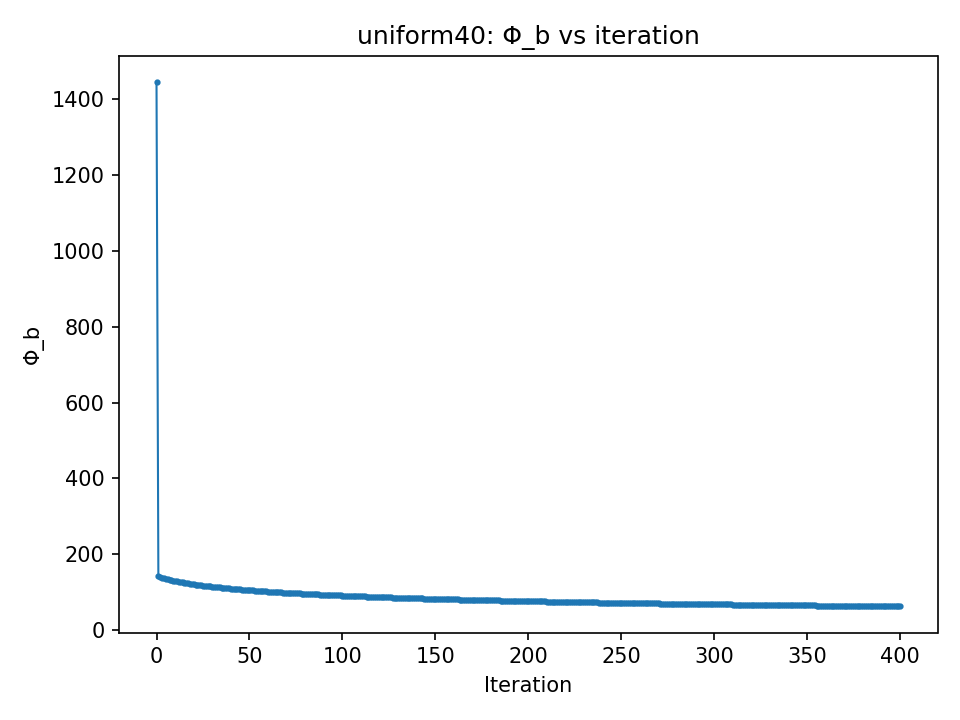
\includegraphics[width=0.32\linewidth]{figures/uniform40_dx0.01_phib_vs_iter.png}
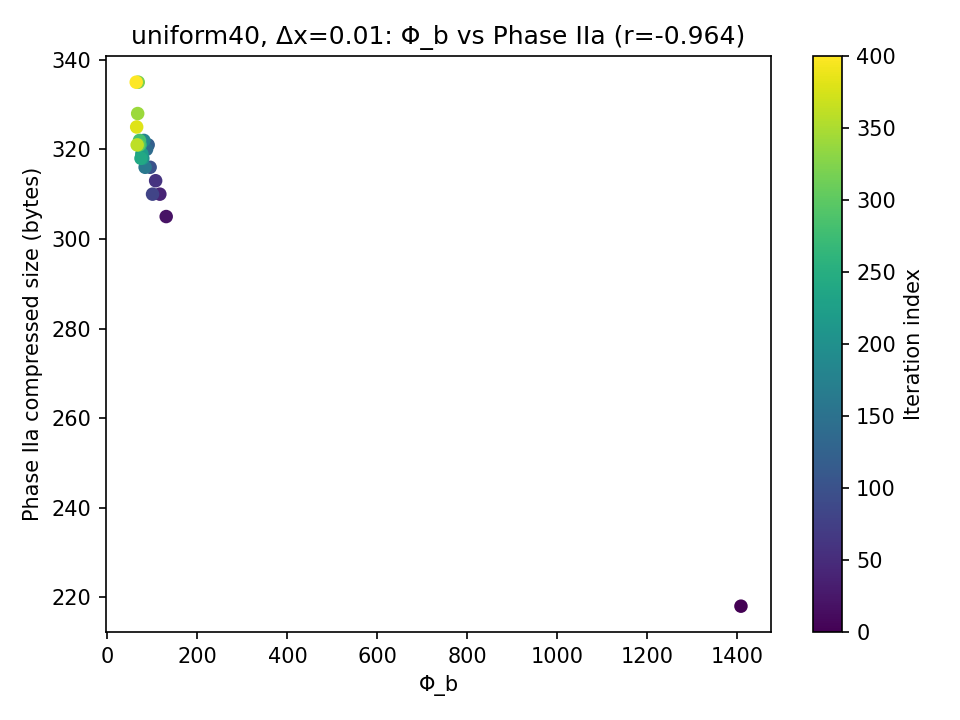
\includegraphics[width=0.32\linewidth]{figures/uniform40_dx0.01_phib_vs_phase2a.png}
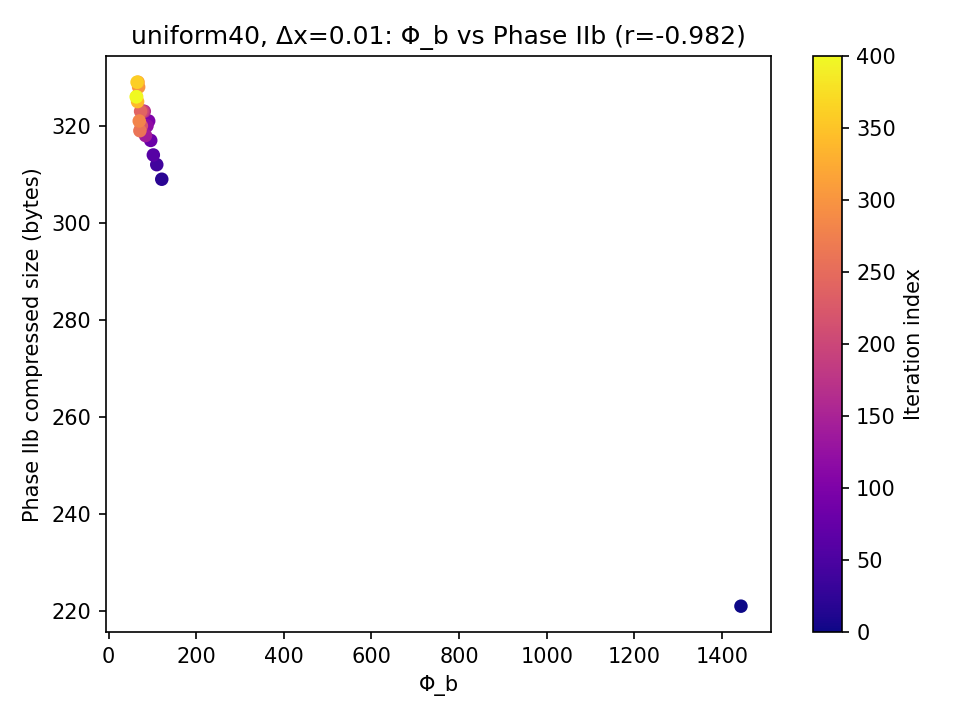
\includegraphics[width=0.32\linewidth]{figures/uniform40_dx0.01_phib_vs_phase2b.png}
\caption{\textbf{Uniform40} ($\Delta x{=}10^{-2}$). Monotone $\phib$ descent and strong co-movement with gzip-compressed size (Phase IIa/IIb).}
\end{figure}

\begin{figure}[htbp]
\centering
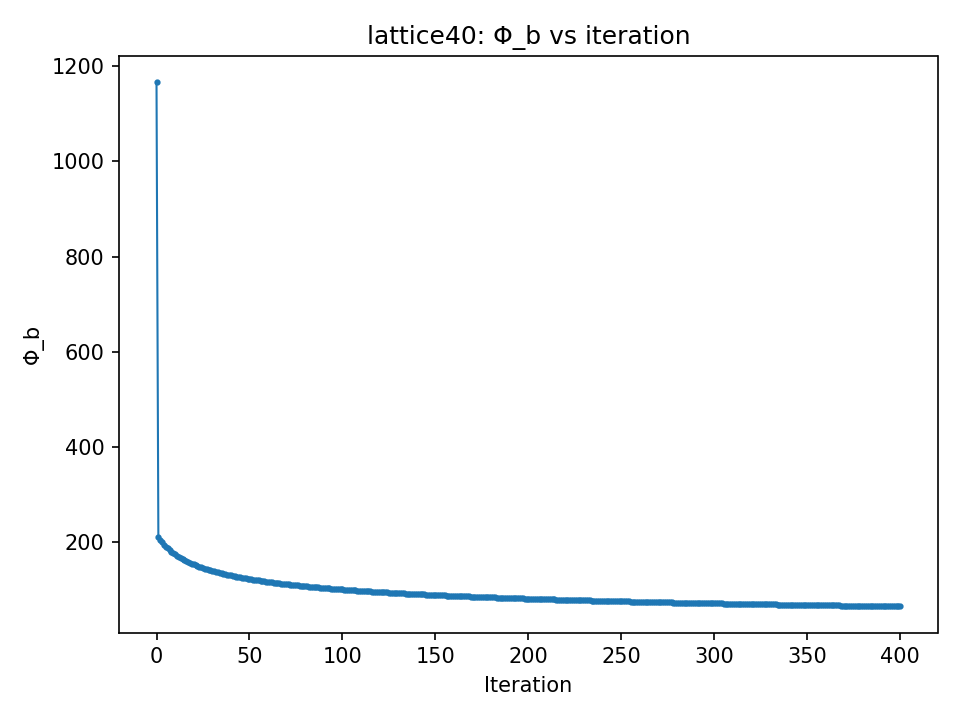
\includegraphics[width=0.32\linewidth]{figures/lattice40_dx0.01_phib_vs_iter.png}
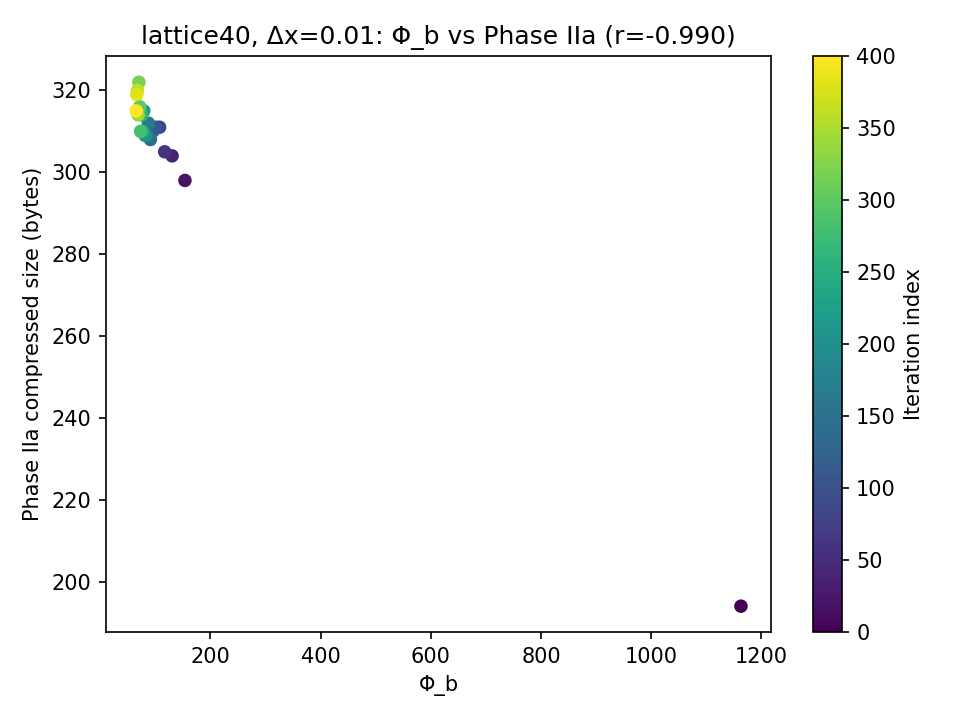
\includegraphics[width=0.32\linewidth]{figures/lattice40_dx0.01_phib_vs_phase2a.png}
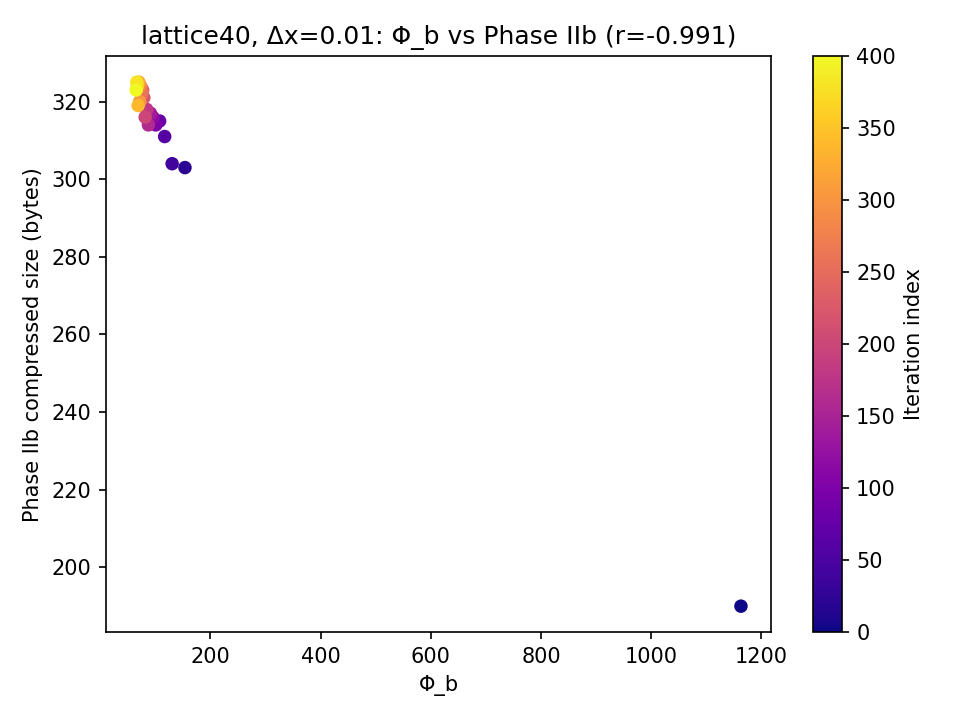
\includegraphics[width=0.32\linewidth]{figures/lattice40_dx0.01_phib_vs_phase2b.png}
\caption{\textbf{Lattice40} ($\Delta x{=}10^{-2}$). Plateaus and weaker correlations; flagged as a rejection case under F3.}
\end{figure}

\begin{figure}[htbp]
\centering
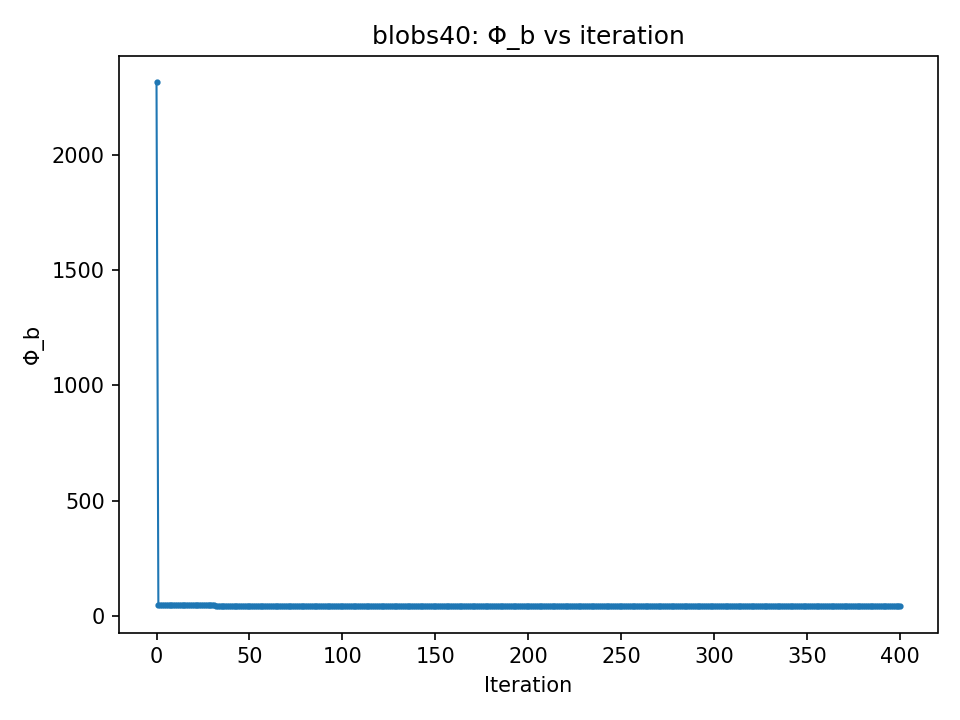
\includegraphics[width=0.32\linewidth]{figures/blobs40_dx0.01_phib_vs_iter.png}
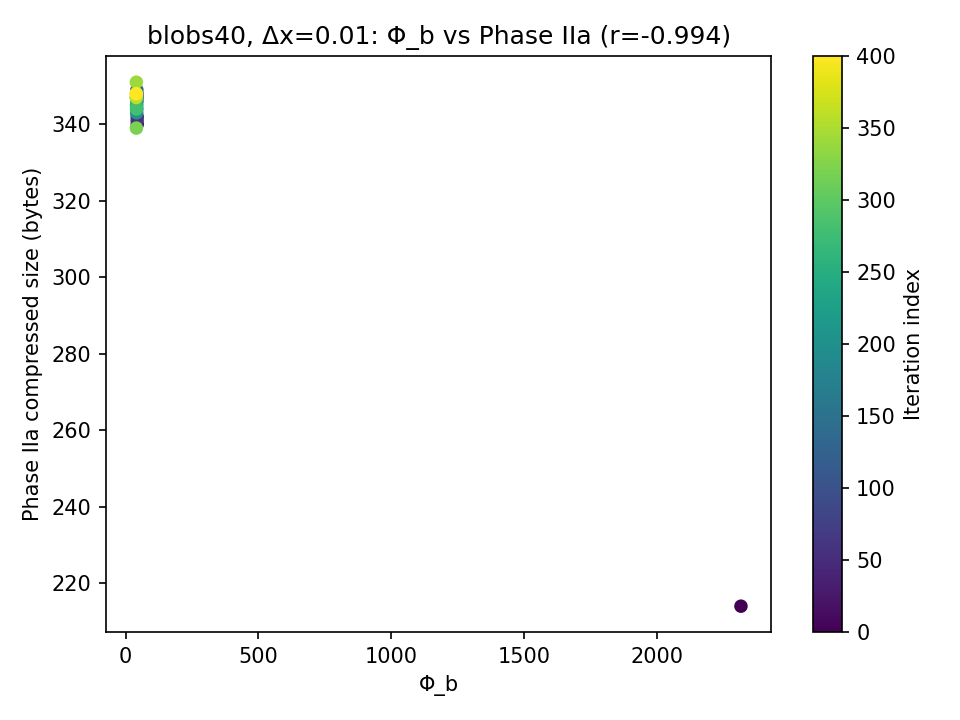
\includegraphics[width=0.32\linewidth]{figures/blobs40_dx0.01_phib_vs_phase2a.png}
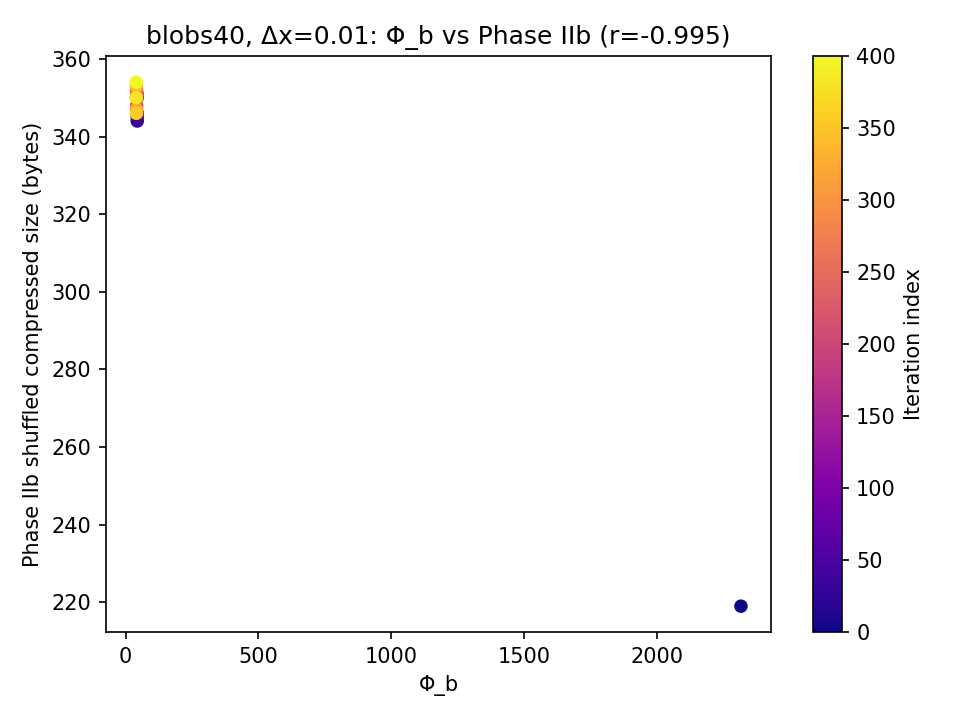
\includegraphics[width=0.32\linewidth]{figures/blobs40_dx0.01_phib_vs_phase2b.png}
\caption{\textbf{Blobs40} ($\Delta x{=}10^{-2}$). Strong monotone link between $\phib$ and gzip bytecount across encoders.}
\end{figure}

\begin{figure}[htbp]
\centering
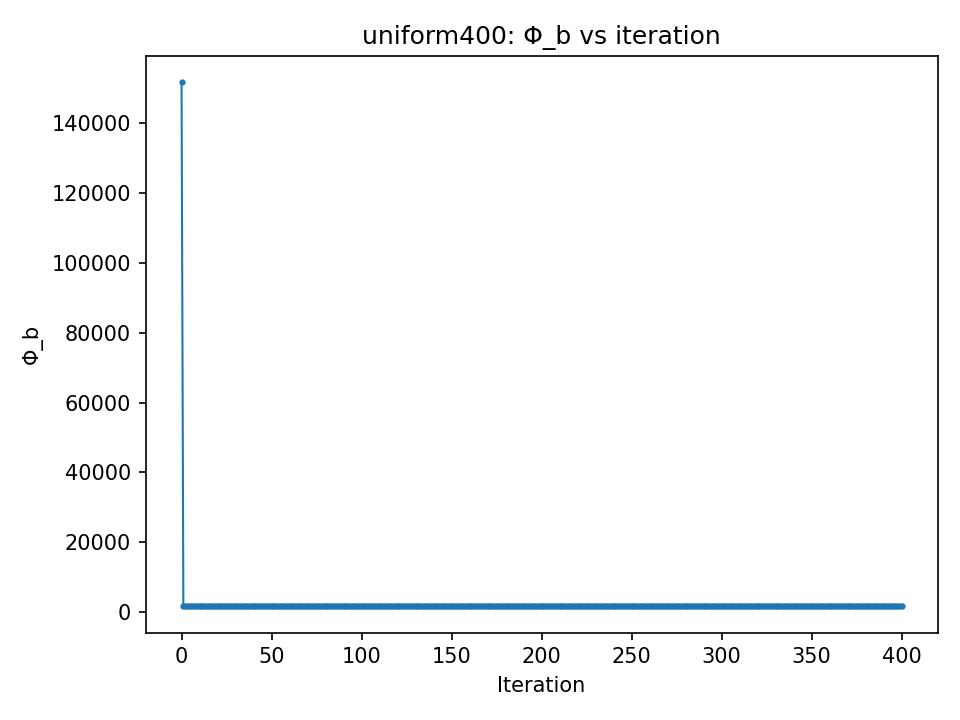
\includegraphics[width=0.32\linewidth]{figures/uniform400_dx0.001_phib_vs_iter.png}
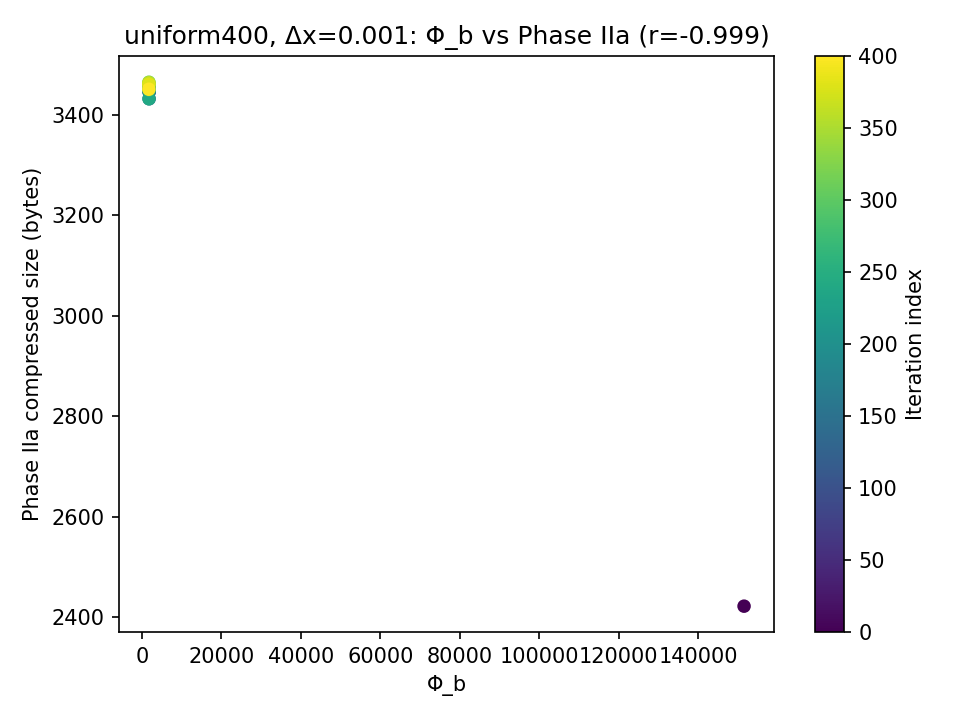
\includegraphics[width=0.32\linewidth]{figures/uniform400_dx0.001_phib_vs_phase2a.png}
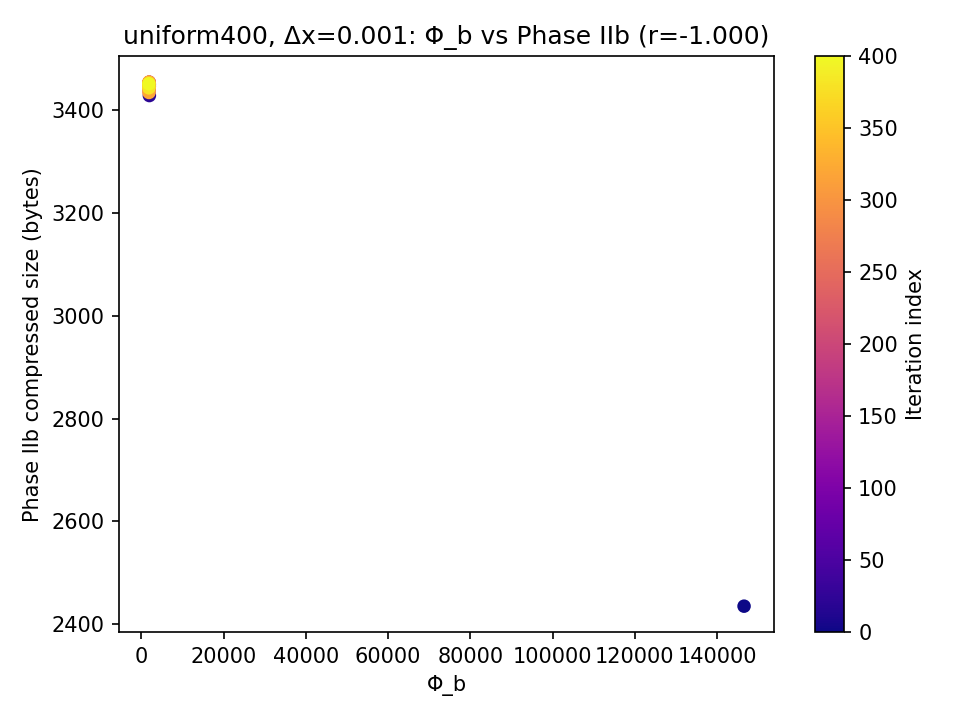
\includegraphics[width=0.32\linewidth]{figures/uniform400_dx0.001_phib_vs_phase2b.png}
\caption{\textbf{Uniform400} ($\Delta x{=}10^{-3}$).  Large-$N$ ensemble with near-perfect co-movement of $\phib$ and gzip bytecount.}
\end{figure}

\section{Results and Interpretation}
\textbf{Scope of claims.}  
The results should be read as an internal audit of a single surrogate along the trajectories it generates.  We do not claim $\phib$ universally predicts compressibility, nor that gzip size measures Shannon entropy.  The narrower statement: during controlled descent, $\phib$ and gzip-compressed coordinate size co-move with high effect size in several ensembles and fail in others.

In \texttt{uniform40}, \texttt{blobs40}, and \texttt{uniform400}, correlations exceed $|r|\!\approx\!0.9$; in \texttt{lattice40} they fall below the preregistered bar, marking a valid rejection.

\subsection*{Failure Analysis: \texttt{lattice40}}
\texttt{lattice40} begins near an ordered packing with low gzip bytecount and low $\phib$.  Descent leaves little dynamic range, so $\eta$ repeatedly shrinks and accepted steps yield minimal change.  $\phib$ and bytecount both plateau, giving modest, noisy correlations.  F3 therefore correctly reports a rejection.  This is a designed outcome: a falsifier must also reject stable or already-ordered configurations.

\section{Model Card (Preregistered Parameters)}
\begin{itemize}
\item System: $N{=}40,400$; seed 0; open boundaries.
\item Functional: $\phib$ of \cref{eq:phib-def}, $a{=}0.05$.
\item Descent: backtracked gradient ($\eta_0{=}0.05$, shrink 0.5, floor $10^{-6}$).
\item Snapshots: every 5 accepted steps.
\item Quantization: $\Delta x\in\{10^{-1},10^{-2},10^{-3}\}$.
\item Encoders: Phase I (64 radial bins + gzip lvl 6), Phase IIa/IIb (quantized coords + gzip lvl 6).
\item Baselines: radius of gyration, mean nearest neighbor distance, coordinate variance.
\item Falsifier: reject if all $|r|<0.7$ on subsampled snapshots.
\end{itemize}

\section{Limitations and Next Steps}
\paragraph{Statistical power.}
Each ensemble uses one seed and $n_{\text{eff}}\!\approx\!21$ snapshots.  $r$ is an effect size, not an inference.  Future work: replicate across many seeds, compute bootstrap confidence intervals, and report distributions of $r$.

\paragraph{Compressor choice.}
gzip measures byte-pattern redundancy after quantization; it is not a principled entropy estimator.  Our claim is limited to gzip: “descending $\phib$ increases byte-level regularity under gzip.”  Extensions: arithmetic coders, learned compressors, $k$-NN or PCA-based entropy estimates.

\paragraph{Causality and out-of-distribution tests.}
This work audits self-consistency along $\phib$-driven trajectories.  Testing prediction across arbitrary states requires evaluating $\phib$ on systems evolved by other potentials or drawn from different ensembles—future work.

\paragraph{Alternative surrogates.}
$\phib$ is one computable choice.  PCD generalizes: any proposed surrogate can be tested under the same falsifier, producing quantitative rejection or support.

\paragraph{Interpretation of F3.}
The $|r|\ge0.7$ bar is heuristic, not inferential.  It functions as an engineering threshold defining a “strong linear link” for this workflow.

\paragraph{Scaling.}
At $N{=}400$, the correlation between $\phib$ and gzip bytecount approaches unity, persisting under coordinate shuffling.  Larger $N$ and multi-seed studies will test generality.

\section{Relation to Prior Work}
PCD connects:
\begin{itemize}
\item Gradient-flow and force-directed methods;
\item Minimum-Description-Length and compression heuristics;
\item Explicit falsifiability and preregistration in surrogate auditing.
\end{itemize}
It provides a reproducible audit harness for computable “compression-pressure” surrogates.

\section{Conclusion}
PCD defines a reproducible, falsifiable loop:
\begin{enumerate}[label=(\arabic*)]
\item choose a computable surrogate $\phib$;
\item evolve a system by monotone descent;
\item record gzip-based and histogram-based bytecounts;
\item sweep quantization $\Delta x$ and compare with geometric baselines;
\item apply F3 and record acceptance or rejection per ensemble.
\end{enumerate}
Some ensembles show high effect sizes, others fail—by design.  
PCD thus functions as an empirical audit template for “compression-pressure” surrogates.

\section*{Acknowledgments}
We thank reviewers for insisting on ordering controls, quantization sweeps, baselines, temporal subsampling, and preregistration.  
Any remaining eccentricities are the author’s own.

\bibliographystyle{plain}
\begin{thebibliography}{10}

\bibitem{Shannon1948}
C.~E.~Shannon.
\newblock A mathematical theory of communication.
\newblock {\em Bell System Technical Journal}, 27:379--423, 623--656, 1948.

\bibitem{Rissanen1978}
J.~Rissanen.
\newblock Modeling by shortest data description.
\newblock {\em Automatica}, 14(5):465--471, 1978.

\bibitem{LeimkuhlerMatthews2016}
B.~Leimkuhler and C.~Matthews.
\newblock {\em Molecular Dynamics}.
\newblock Springer, 2016.

\bibitem{Wendland1995}
H.~Wendland.
\newblock Piecewise polynomial, positive definite and compactly supported radial functions.
\newblock {\em Adv. Comput. Math.}, 4:389--396, 1995.

\bibitem{FruchtermanReingold1991}
T.~M.~J. Fruchterman and E.~M.~Reingold.
\newblock Graph drawing by force-directed placement.
\newblock {\em Software: Practice and Experience}, 21(11):1129--1164, 1991.

\end{thebibliography}

\end{document}
